%%%%%%%%%%%%%%%%%%%%%%% file template.tex %%%%%%%%%%%%%%%%%%%%%%%%%
%
% This is a template file for Web of Conferences Journal
%
% Copy it to a new file with a new name and use it as the basis
% for your article
%
%%%%%%%%%%%%%%%%%%%%%%%%%% EDP Science %%%%%%%%%%%%%%%%%%%%%%%%%%%%

\documentclass{webofc}
% option "twocolumn" for typesetting an article in two columns format (default one column)
% \documentclass[twocolumn]{webofc}

\usepackage[varg]{txfonts}   % Web of Conferences font
\usepackage{hyperref}
\usepackage{url}
\usepackage{minted}
%%%%%%%%%%%%%%%%%%%%%%%%%%%%%%%%%%%%%%%%%%%%%%%%%%%%%%%%%%%%%%%%%%%%%%%%%%%%%
\hypersetup{colorlinks=true,citecolor=blue,urlcolor=blue,linkcolor=blue}
%%%%%%%%%%%%%%%%%%%%%%%%%%%%%%%%%%%%%%%%%%%%%%%%%%%%%%%%%%%%%%%%%%%%%%%%%%%%%
%
% Put here some packages required or/and some personnal commands
%
%
\begin{document}
%
\title{A new SymPy backend for Vector: uniting experimental and theoretical physicists}
%
% subtitle is optionnal
%
%%%\subtitle{Do you have a subtitle?\\ If so, write it here}


\author{\firstname{Saransh} \lastname{Chopra}\inst{1}\fnsep\inst{2} \and
        \firstname{Jim} \lastname{Pivarski}\inst{2}\fnsep\thanks{\email{pivarski@princeton.edu}}
}

\institute{University College London 
\and
           Princeton University 
          }

\abstract{Vector is a Python library for 2D, 3D, and Lorentz vectors, especially arrays of vectors, to solve common physics problems in a NumPy-like way. Vector can currently perform numerical computations, and through this paper, we introduce a new symbolic backend that extends Vector's utility to theoretical physicists. The numerical backends of Vector enable users to create pure Python object, NumPy arrays, and Awkward arrays of vectors. The object and Awkward backends are also implemented in Numba to leverage Just-In-Time (JIT) compiled vector calculations. The new symbolic backend, built on top of SymPy expressions, showcases Vector's ability to support far-flung cases and allows SymPy methods and functions to work on vector classes. Moreover, apart from a few software, high energy physics has maintained a strict separation between tools used by theorists and experimentalists, and Vector's SymPy backend aims to bridge this gap, providing a unified computational framework for both communities.
}
%
\maketitle
%
\section{Introduction}
\label{intro}

The Scikit-HEP \cite{scikit-hep} ecosystem was primarily designed to be used by experimental physicists to manipulate and perform physics analysis on numerical data. Theoretical physicists have had limited engagement with Scikit-HEP and other experimental physics frameworks, as there exists a divide between the software used by them and experimental physicists. Moreover, only MC generators like Pythia \cite{pythia} are routinely used by both groups, and there have been little to no efforts to unify the software used by theorists and experimentalists.

Vector was designed from the ground up to have multiple computational backends. The core compute functions of the library are written to be generic and library-agnostic, such that they operate only on the data containers and not the data itself. This design pattern has already led to the development of Vector's three backends -

\begin{itemize}
    \item the object backed for vectors that pure Python objects,
    \item the NumPy \cite{harris:2020} backend for NumPy arrays of vectors,
    \item the Awkward \cite{Pivarski:2018} backend for Awkward arrays of vectors,
\end{itemize}

\noindent and Numba \cite{lam:2015} extensions for the object and Awkward backends.

All three backends share the same duck-typed compute functions, allowing Vector to increase the number of backends without adding explicit compute functions for each of them. Therefore, this paper extends Vector to operate on symbolic, or SymPy \cite{Meurer:2017}, expressions to showcase the diversity of backends it can scale to and to enable both experimental and theoretical physicists to utilize the library in their work. Since the SymPy vector classes and their momentum equivalents operate on SymPy expressions, all of the standard SymPy methods and functions work on the vectors, vector coordinates, and the results of operations carried out on vectors. Moreover, Vector’s SymPy backend aims to create a stronger connection between software used by experimentalists and software used by theorists.

\section{Implementation}
\label{sec-implementation}

Vector's design and duck typing of compute functions (allowing them to be shared amongst the backends) paved the way for the development of the SymPy backend. The SymPy backend's implementation consists of coordinate and vector classes that are capable of constructing vectors using SymPy's data containers and wrapping compute function results as SymPy expressions.

Figure \ref{fig:sympy} shows how the SymPy backend and other Vector backends interact with the compute functions. Each backend has its own coordinate and vector classes that can accept numerical (for the case of object, NumPy, and Awkward backend) or symbolic (for the case of SymPy backend) arguments. The classes, as well as their methods, are compatible with the respective backend libraries. The object and Awkward backends use NumPy to perform all the arithmetic, and Awkward Array internally maps the NumPy calls to custom functions for ragged arrays.

\begin{figure}[h]
     \centering
     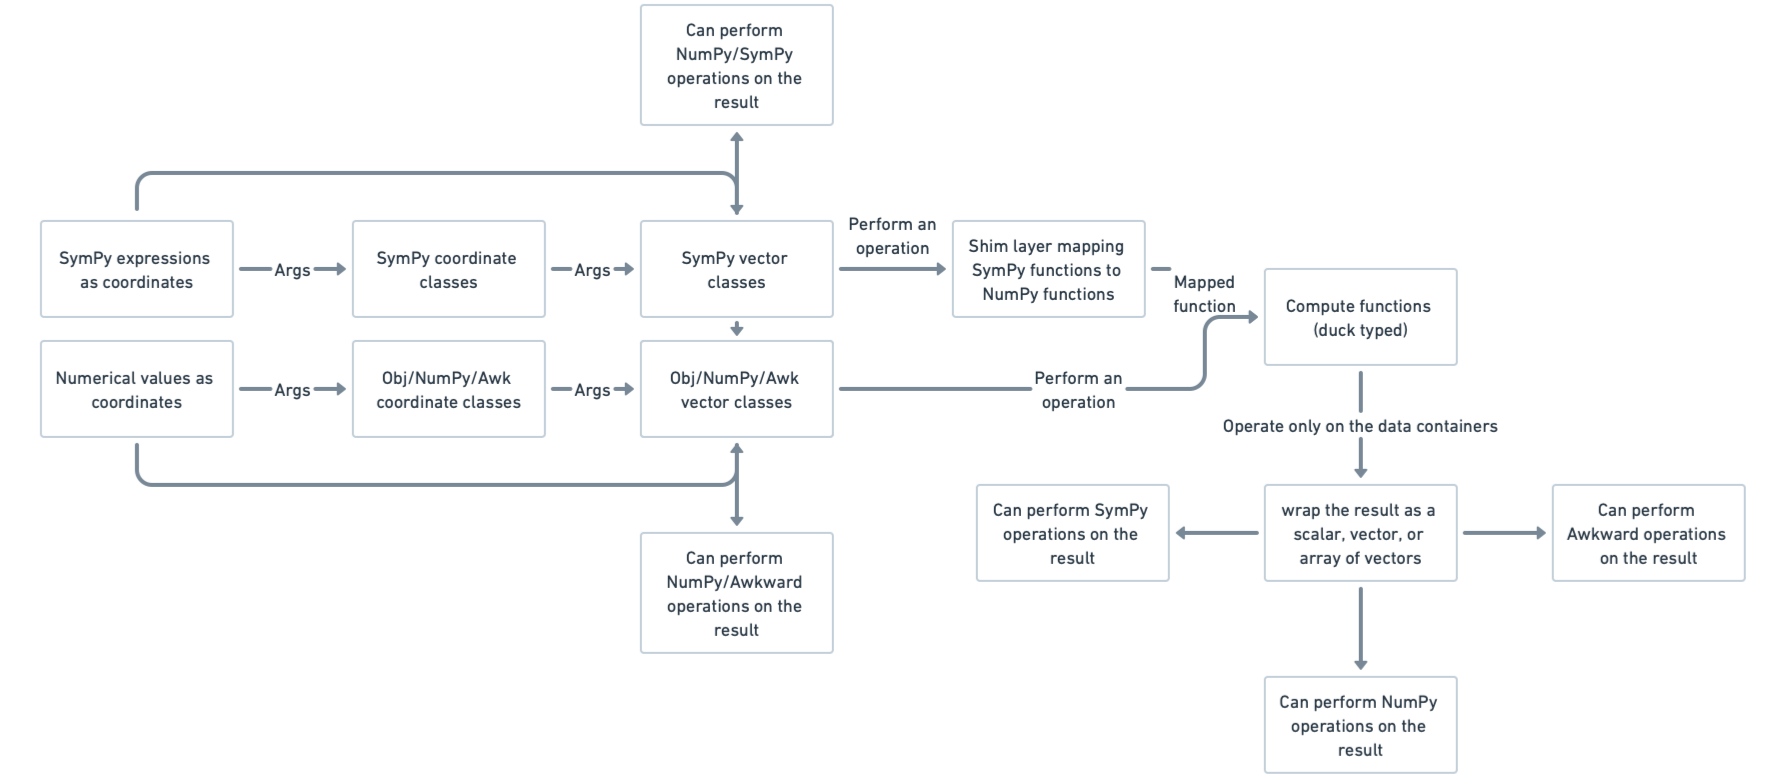
\includegraphics[width=\textwidth]{sympy-backend.png}
     \caption{Implementation of Vector's SymPy backend.}
        \label{fig:sympy}
\end{figure}

Finally, all the compute functions valid on the dimension of the constructed vector work with all the backends. At the moment, the compute functions switch between backend libraries using a shim layer. This shim layer is not required for the object, NumPy, and Awkward backends because NumPy works with all of them. On the other hand, due to different naming conventions between SymPy and NumPy, the NumPy functions are mapped to the respective SymPy functions in the shim layer and are flown down to the compute functions. The results from these compute functions are wrapped with values or appropriate data structures in the vector classes. This wrapped result can then be used in any of the functions provided by the backend libraries, making a strong cohesion between Vector backends and the backend libraries.

\section{Demonstration}
\label{sec-demonstration}

Consider the example \ref{vector-obj} performing \mintinline{python}{deltaR} operation on two object type 4D Momentum vectors.

\begin{listing}[!ht]
\begin{minted}{python}
import vector

muon_1_obj = vector.MomentumObject4D(px=1, py=2, pz=3, E=10)
muon_2_obj = vector.MomentumObject4D(px=2, py=3, pz=4, E=11)

muon_1_obj.deltaR(muon_2_obj)
# 0.19249147660266414
\end{minted}
\caption{Performing deltaR on object vectors.}
\label{vector-obj}
\end{listing}

The exact same operation can be carried out using the SymPy backend with an almost identical syntax. Example \ref{vector-sympy} shows how SymPy \mintinline{python}{symbols} can be passed into \mintinline{python}{MomentumSymPy} as arguments just like numerical values are passed into \mintinline{python}{MomentumObject}. The \mintinline{python}{deltaR} operation on the SymPy vector returns a SymPy expression instead of a numerical value. The obtained SymPy expression is compatible with every SymPy method and function; hence, one can substitute (\mintinline{python}{subs}) and evaluate (\mintinline{python}{evalf}) the resultant expression to validate the theoretical expression.

\begin{listing}[!ht]
\begin{minted}{python}
import vector; import sympy

px_1, py_1, pz_1, E_1 = sympy.symbols(
    "px_1 py_1 pz_1 E_1", real=True
)
px_2, py_2, pz_2, E_2 = sympy.symbols(
    "px_2 py_2 pz_2 E_2", real=True
)

muon_1_sympy = vector.MomentumSympy4D(
    px=px_1, py=py_1, pz=pz_1, E=E_1
)
muon_2_sympy = vector.MomentumSympy4D(
    px=px_2, py=py_2, pz=pz_2, E=E_2
)

muon_1_sympy.deltaR(muon_2_sympy)
# sqrt((Mod(atan2(py_1, px_1) - atan2(py_2, px_2) + pi, 2*pi)
# - pi)**2 + (asinh(pz_1/sqrt(px_1**2 + py_1**2))
# - asinh(pz_2/sqrt(px_2**2 + py_2**2)))**2)

# take the values from object type vectors
muon_1_sympy.deltaR(muon_2_sympy).subs(
    {
        px_1: muon_1_obj.px,
        py_1: muon_1_obj.py,
        pz_1: muon_1_obj.pz,
        E_1: muon_1_obj.E,
        px_2: muon_2_obj.px,
        py_2: muon_2_obj.py,
        pz_2: muon_2_obj.pz,
        E_2: muon_2_obj.E,
    }
).evalf()
# 0.192491476602664
\end{minted}
\caption{Performing deltaR on SymPy vectors.}
\label{vector-sympy}
\end{listing}

Furthermore, \ref{vector-sympy-extra} depicts how some of the other SymPy functionalities - using \mintinline{python}{simplify} to simplify expressions and converting expressions into code for a particular programming language - can be called on the symbolic results.

\begin{listing}[!ht]
\begin{minted}{python}
import vector; import sympy

x, y, z, t = sympy.symbols(
    "x y z t", real=True
)

v = vector.VectorSympy4D(x=x, y=y, z=z, t=t)

v.boost(v.to_beta3()).t
# t/sqrt(1 - x**2/t**2 - y**2/t**2 - z**2/t**2) + x**2/(t*
# sqrt(1 - x**2/t**2 - y**2/t**2 - z**2/t**2)) + y**2/(t*
# sqrt(1 - x**2/t**2 - y**2/t**2 - z**2/t**2)) + z**2/(t*
# sqrt(1 - x**2/t**2 - y**2/t**2 - z**2/t**2))

v.boost(v.to_beta3()).t.simplify()
# t*sqrt((t**2 - x**2 - y**2 - z**2)/t**2)*(t**2 + x**2 +
# y**2 + z**2)/(t**2 - x**2 - y**2 - z**2)

import sympy.printing.c

print(sympy.printing.c.ccode(boosted.t.simplify()))
# t*sqrt((pow(t, 2) - pow(x, 2) - pow(y, 2) - pow(z, 2))/
# pow(t, 2))*(pow(t, 2) + pow(x, 2) + pow(y, 2) + pow(z, 2))
#/(pow(t, 2) - pow(x, 2) - pow(y, 2) - pow(z, 2))
\end{minted}
\caption{Simplifying expressions and converting expressions into code for another programming language.}
\label{vector-sympy-extra}
\end{listing}

\section{Challenges}
\label{sec-challenges}

The symbolic backend has two minor but intentional caveats. SymPy internally uses mpmath \cite{mpmath} to perform complex floating-point arithmetic, leading to minor disagreements between the results obtained through the numerical (object, NumPy, and Awkward) and the symbolic backends. This disagreement can be minimized by specifying more decimal points in the precision. Further, operations on SymPy vectors are only 100\% compatible with numeric vectors if the vectors are positive time-like, that is, if the following inequality

\begin{equation} \label{ineq-positive-time}
t^{2} > x^{2} + y^{2} + z^{2}
\end{equation}

\noindent where $x$ and $y$ are Cartesian azimuthal coordinates, $z$ is Cartesian longitudinal coordinate, and $t$ is Cartesian time, holds true. The space-like and negative time-like cases have different sign conventions, which would have led to \mintinline{python}{if-else} statements in the code, making it impossible for SymPy to simplify symbolic expressions. Hence, to make SymPy's simplifications work, space-like and negative time-like sign conventions are ignored in the shim layer. Given that most high energy physics analyses deal with positive time-like vectors, this caveat does not hinder the ability to use Vector's SymPy backend in theoretical calculations.

\section{Future work}
\label{sec-future-work}

The SymPy backend offers users several new features, some of which are relatively under-explored. Symbolic differentiation and code generation for other languages are two such important but unexplored features.

On one hand, there has been a recent push to make high energy physics analysis pipelines differentiable for parameter tuning, such as the ongoing work on integrating Automatic Differentiation in the Analysis Grand Challenge \cite{Held:2022sfw}. Vector already extends the JAX \cite{Bradbury:2018} backend of Awkward Array, and with the development of SymPy backend, Vector can be expected to perform both automatic and symbolic differentiation. On the other hand, code generation for another language through the SymPy backend can potentially help physicists flexibly switch languages and frameworks for their analyses. Both of these functionalities can be assessed and experimented with in the future to fill gaps in the software used for high energy physics.

\section{Acknowledgements}
\label{sec-acknowledgements}

The work on Vector's symbolic backend was supported by NSF cooperative agreements OAC-1836650 and PHY-2323298 (IRIS-HEP).

\bibliography{cites.bib}
\end{document}

% end of file template.tex

<div id='footer'><table width='100%'><tr><td class='right'><a href='http://fusioninventory.org/'><span class='copyright'>FusionInventory 9.1+1.0 | copyleft <img src='/glpi/plugins/fusioninventory/pics/copyleft.png'/>  2010-2016 by FusionInventory Team</span></a></td></tr></table></div>